\documentclass[a4paper, 12pt]{article}
\usepackage[utf8]{inputenc} % Allows for special characters
\usepackage{graphicx} % For including images
\usepackage{amsmath} % For mathematical symbols
\usepackage{hyperref} % For hyperlinks
\usepackage{geometry} % For page layout
\geometry{margin=1in} % Adjust margins


\begin{document}
% Front Page
\begin{titlepage}
    \begin{center}
        % University Logo
        
\includegraphics[width=0.2\textwidth]{uovlogo.png} \\[1cm]

        % Title
        \textbf{\LARGE \textbf{IT3162 Group Project}} \\[1cm]

         \textbf{\LARGE ElderCare Connect} \\[1.5cm]
        % Subtitle (optional)
        \textbf{{\Large Group I}} \\[1cm]
        \begin{tabular}{ll}
            \large Ms. Indrejith S.A.C.S.       & \large 2020/ICT/65 \\ [0.5cm]
            \large Ms. Perera H.D.S             & \large 2020/ICT/91 \\ [0.5cm]
            \large Ms. Lakmini L.A.M.           & \large 2020/ICT/44 \\ [0.5cm]
            \large Ms. Thavarajah H.            & \large 2020/ICT/120 \\ [0.5cm]
            \large Ms. Chandrasekara C.G.H.P.L. & \large 2020/ICT/69 \\ [0.5cm]
            \large Ms. Lakshna G.               & \large 2020/ICT/83 \\ [0.5cm]
            \large Mr. Imran B.M.               & \large 2020/ICT/02 \\ [1.5cm]
        \end{tabular}

        \textbf{\Large Supervised by:} \\ [0.5cm]
        \large Mr. K. Mathanaharan \\[1.5 cm]

        \textbf{\Large Department of Physical Science} \\ [0.25cm]
        \textbf{ \Large Faculty of Applied Science} \\ [0.25cm]
        \textbf{\Large University of Vavuniya} \\ [0.25cm]
        \textbf{\Large October 2024} \\ [0.25cm]

       
    \end{center}
\end{titlepage}

\section{\textbf{\LARGE Introduction}}
\subsection{\textbf{\Large Introduction}}

Elderly individuals who live alone face significant health and safety challenges, including medical emergencies, falls, and feelings of isolation. Due to the lack of immediate assistance, these incidents can lead to delayed medical attention and complications. Furthermore, isolation can negatively affect their mental and emotional health. The absence of regular check-ins and health tracking increases the risk of undetected health deterioration.

The project aims to help develop a Progressive Web Application (PWA) designed to enhance the safety, health monitoring, and social well-being of elderly individuals living alone. Through tracking real-time health (using APIs like Google Fit), the app will ensure caregivers/family members can monitor their health status from a distance .

The ElderCare Connect will function across multiple devices (desktops, smartphones, and tablets) with native app-like experiences, providing real-time health monitoring, emergency alerts, and social engagement features.  Push notifications will ensure immediate attention during emergencies. Messaging features will help elderly connected with family, friends, and caregivers, mitigating loneliness and providing emotional support with PWA advantages. Data security and privacy are top priorities.

\subsection{\textbf{\Large Objectives}}

The main aim of this project is to facilitate all-encompassing support for elderly living alone by introducing an accessible Progressive Web Application (PWA) integrating health monitoring, emergency response and social engagement services.
The app will use wearable devices to provide caregivers and family members with real-time data on the health status of a user, while also adopting a third-party API such as Google Fit.
For medical emergencies, the app will alert caregivers or emergency services immediately so that they can provide immediate help.
It will also include a social interaction component to eradicate loneliness by allowing users the ability to communicate with family and friends as well.
While achieving data security and privacy, the project also targets seamless user experience as we add offline capability while push notifications will be a top priority, with robust authentication and encryption methods in place to safeguard sensitive user information.

\subsection{\textbf{\Large Benefits of this Research}}

The benefits of this research extend beyond immediate health monitoring and emergency response; it significantly enhances the overall well-being of elderly individuals living alone. By providing real-time tracking of vital signs through wearable technology, the project could reduce hospitalizations and prevent severe medical conditions from escalating. In addition to that, by medication reminders elderly users will not forget their daily dose of medicines.
The integration of emergency alert systems ensures rapid intervention during critical situations, potentially lowering mortality rates and long-term complications. Social engagement features address the mental health challenges associated with loneliness and social isolation, which are common among the elderly, thus improving their emotional resilience and quality of life.
The research promotes the development of secure and scalable digital health solutions, ensuring that sensitive health data is protected through robust security measures. It paves the way for future innovations in elderly care technology, setting a precedent for more advanced applications that can be used in home-based and institutional care environments. From the caregivers and family’s perspective, this research provides peace of mind, offering a reliable, real-time method of staying connected with their loved ones' health and safety.

\subsection{\textbf{\Large Background}}

In recent decades, smartphones have significantly changed the way we live. In terms of the health sector, elderly individuals now have greater access to health information and can enhance the convenience of managing their medical care through mobile applications. Several studies have shown the positive impact of mobile health interventions in managing lifestyle factors such as improving diet, quitting smoking, and increasing physical activity, as well as controlling chronic conditions like diabetes and hypertension. This change has also influenced the relationship between patients and their general practitioners.

Recent research has shown that patients see mobile health apps as valuable tools for self-monitoring and self-managing their own health. However, they also acknowledge certain limitations, such as issues with battery life and concerns regarding the legal aspects of electronic prescribing.

Moreover, there has been increasing concern regarding the rising number of elderly individuals, particularly those living alone due to the population ageing across the globe. This demographic group faces great challenges, including high health risks, social disconnectedness, and slow responses in case of emergencies that may endanger their lives. Considering that such a severe future scenario would likely occur much faster than a call for help or even faster than some normal medical conditions, there is a need for solutions that can protect the elderly, particularly those without nearby family members, from possible future threats.

\subsubsection{\textbf{\large Threats to the Lives of Elderly Living Alone}}

Some common venture medical emergencies include the sudden health collapse experienced by many elderly people with chronic diseases such as heart conditions, diabetes, or even mobility problems. Most times, these medical emergencies occur when the elderly are alone, and this results in treatment being delayed which ultimately leads to worse outcomes.

Falls are inherent dangers for the elderly and statistical data among this age group shows that these occurrences are frequent in old age. When an elderly individual does not receive services, or assistance immediately after suffering a fall, it can lead to serious consequences such as bone fractures or head trauma and in some cases may end with being bedridden for long periods of time.
Several studies have already shown the relationship between social isolation and the moral health of elderly people, leading either to depression or dementia. In addition to that, such self-imposing isolation because of scarcity of social contact may also prevent a person from leading a healthy life or postpone a visit to a medical doctor when required.

\subsection{\textbf{\Large Literature Review and Scope}}
\subsubsection{\textbf{\large Literature Review}}

Existing technological solutions for the elderly have a tendency to address very distinct elements of support while failing to offer a completely holistic and integrated experience. LifeFone, a medical monitoring device with emergency alerts, enables swift help in case of medical emergencies, such as falls or any sort of sudden illness.  MediSafe provides reminders for medicines that can assist the individuals in managing treatment compliance.  Aloe Care offers features such as activity detection and caregiver engagement tools for greater awareness, but it offers minimal services in health status and safety monitoring.

The literature shows that current solutions have been created in separate entities, and therefore there's an absence of a method which will provide seamless connectivity and coordination among these solutions. Health monitoring functionalities are frequently underdeveloped on mobile apps; therefore users don’t have a complete picture of their wellbeing.  Communication tools might also be missing and are necessary for the prevention of senior isolation, depression and an active engagement inside a supportive community.   These current products often lack user friendly interfaces, which are essential for people who may have difficulty with computers and may not be familiar with it.

\subsubsection{\textbf{\large Scope}}

The ElderlyCare Connect project's scope involves the building of a PWA which provides seniors living independently complete features for health, and connectivity, which ensures their safety and social engagement. Wearable sensor applications are to be used for continuous monitoring of vital parameters like the heart rate, blood pressure and activity level, thus permitting quick detection of issues needing quick actions. As a support measure, there's an immediate alert feature which instantly notifies the caregivers as well as the emergency teams, helping guarantee that support will be sent rapidly during critical times. Messaging features and location tracking also will be included. The project prioritizes user-friendly design for seniors.
 
\subsection {\textbf{\Large Problem Statement}}
Elderly individuals living alone face a confluence of interconnected problems that significantly compromise their well-being. While there are existing systems to assist in distinct areas such as emergency help and medications compliance, these solutions usually fail to give a complete approach that addresses diverse and interconnected requirements of seniors.

There is an issue because often have delayed medical responses can be a vital issue. Medical emergencies that involves falls or stroke can prove detrimental when medical response is slow, which leads to severe consequences such as disability or, worse, loss. Existing emergency systems need improvements on how they can be improved. Seniors can't always be certain about their situations, since sudden medical issues, such as paralysis or serious mental condition, can render them incapable of activating those alerts.

There is one more component that are causing a great risk to elderly individuals, are the isolation and loneliness. This problem has wide implications for physical and mental well-being.
This project is committed to developing an application PWA, to mitigate the issues that current systems have, thus, our commitment to help the seniors is in high regard.

\subsection{\textbf{\Large Proposed Solution}}
The proposed solution, ElderCare Connect, is a Progressive Web Application (PWA) designed to serve as a comprehensive, integrated platform for elderly individuals living alone. We will leverage a range of technologies, in order to address the diverse requirements of these individuals.

First, we will integrate with wearable devices for real-time tracking of vital signs. Through real-time health monitoring systems that utilize wearable devices, such as fitness bands and smart watches, we will be able to monitor critical indications such as heart rate, blood pressure, and their activities over time with high precision. The data will immediately transmit using the PWA, that way caregivers/family can observe it and monitor their health on a continuous basis.

For any critical situations that will be triggered by those seniors, will also give the capability to those caretakers, which enable help as soon as possible. A user-friendly design interface can definitely make a huge difference in making technology more accessible to older people. By incorporating larger text, basic navigation, and visual icons that can be seen as easier compared to traditional apps, the intention of ElderCare Connect is to be naturally integrated into their daily routine. We will also incorporate a wide integration of social features that will include features in messaging, video conferences, forums, and even social activity.

\section{\textbf{\LARGE Requirement Analysis}}
\subsection{\textbf{\Large Introduction}}
In this context of requirement analysis, the ElderCare Connect Progressive web application is designed to meet the needs of specific users such as elderly people and caregivers. The primary focus of the requirement analysis is to define the functional and non-functional requirements of the system. User requirements of the application include Health monitoring, Emergency Response and social engagement and  the non-functional requirements include Performance, usability, reliability, security, scalability, maintainability and availability.

\subsection{\Large User Requirements} 

\textbf{\large Elderly Users} 
\begin{itemize}
    \item \textbf{Health Monitoring:} Integration with wearable devices to track vital signs like heart rate, blood pressure, and physical activity. 
    \item \textbf{Emergency Alerts:} Automatic fall detection and an SOS button for emergencies, sending alerts to family, caregivers, or emergency services.
    \item \textbf{Medication Reminders:} Notifications to take prescribed medications, reducing the risk of missed doses. 
    \item \textbf{Daily Check-ins:} Gentle reminders for users to confirm their well-being or complete a wellness survey.
    \item \textbf{Social Engagement:} Messaging, and virtual communities to reduce isolation and encourage interaction.
\end{itemize}
\textbf{\large Caregivers/family} 
\begin{itemize}
    \item \textbf{Real-time Alerts:} Immediate notifications for falls, emergencies, or missed check-ins.
    \item \textbf{Health Reports:} Weekly or monthly health reports with trends in the user's vital stats, activity levels, and overall well-being.
    \item \textbf{Location Tracking:} Real-time GPS tracking during emergencies or to ensure the user's safety.
    \item \textbf{Communication Tools:} Instant messaging to check on the elderly user.
\end{itemize}

\subsection{Users}
\begin{enumerate}
    \item Caregivers/family
    \item Elderly Users
\end{enumerate}

\subsection{Functional Requirements}
\textbf{Health Monitoring }
\begin{itemize}
    \item The app will be able to synchronize and connect with wearable devices as well as health monitoring platform, Google Fit (Android) which are designed to monitor the heart rate of users, their activity, etc. sleep patterns, their activity levels etc. This data shall be monitored over the internet and in case of any abnormalities such as a distinct drop in heart rate or a fainting episode, alerts will go off. [1]
\end{itemize}
\textbf{Emergency Response}
\begin{itemize}
    \item In the event of a medical emergency or situation where a patient falls, the app shall send push notifications to the emergency contacts or the caregivers who are predesignated. It is also possible for the users to use the emergency call function (with the help of a REST API) in case they feel the need for help or are unwell.
\end{itemize}
\textbf{Social Engagement }
\begin{itemize}
    \item Recognizing the significance of social engagement, which is crucial in enhancing the well-being of the elderly, the only such application will integrate a number of features such as instant messaging where old or elderly users can meet family members, caregivers, which will help in alleviating loneliness and associated feelings. If the elderly member is in danger this features a location sharing technique to send their location to their cared ones. This also allows the family members and caregivers to remind their lovely one’s medications, hydrations and medical consultations simply contact with them.
\end{itemize}
\subsection{Non-functional Requirements}
\textbf{Performance: }
\begin{itemize}
    \item The app should provide real-time monitoring and instant emergency alerts within 2 seconds of a triggering event 95\% of the time, especially during critical moments like falls or health issues.
    \item It should handle multiple users and real-time data input from up to 100,000 wearable devices effectively, maintaining response time of under 1 second per device.
\end{itemize}
\textbf{Usability }
\begin{itemize}
    \item The user interface should be simple and intuitive, designed with large fonts (minimum size 18pt) and easy navigation, particularly catering to elderly users with minimal technical experience (new users will be able to locate easily the primary functions such as emergency alerts, health stats, and alerts within 2 seconds).
    \item The app must be highly reliable to ensure constant monitoring and timely emergency alerts, at least 99.9\% uptime.
    \item Emergency alert mechanisms should function with at least 98\% accuracy, even in low connectivity scenarios (1 Mbps).
\end{itemize}
\textbf{Security }
\begin{itemize}
    \item Data privacy and security are critical, especially since the app deals with sensitive health information. The app must comply with healthcare privacy regulations like HIPAA (or regional equivalents) to protect user data as well as Personal Data Protection Act (PDPA).
    \item Secure login and role-based access for family members and caregivers to ensure only authorized individuals can view the elderly user's health data.
\end{itemize}
\textbf{Scalability }
\begin{itemize}
    \item The back-end should support future scalability as 100\% increase in users and data volume within one year without affecting performance metrics, handle up to 5 million records allowing additional data points (such as vital signs) as needed.
\end{itemize}
\textbf{Maintainability }
\begin{itemize}
    \item The system should be easy to update with new features or improvements, such as new integrations with different wearable devices or additional health monitoring features with maximum downtime of 5 minutes per update.
\end{itemize}
\textbf{Availability }
\begin{itemize}
    \item The system must ensure high availability, especially during emergencies, and maintain uptime for 24/7 real-time monitoring.
    \item Regular maintenance or updates should not interfere with the core emergency functionalities.
\end{itemize}
\textbf{Privacy and Security }
\begin{itemize}
    \item As the application deals with sensitive personal health information, the app will definitely put in place stringent measures such as the use of JWT (JSON Web Tokens) for user validation and SSL which encrypts data during transfer. Such measures go a long way in securing personal health information.
\end{itemize}
\subsection{UseCase Diagram}
\begin{figure}
    \centering
    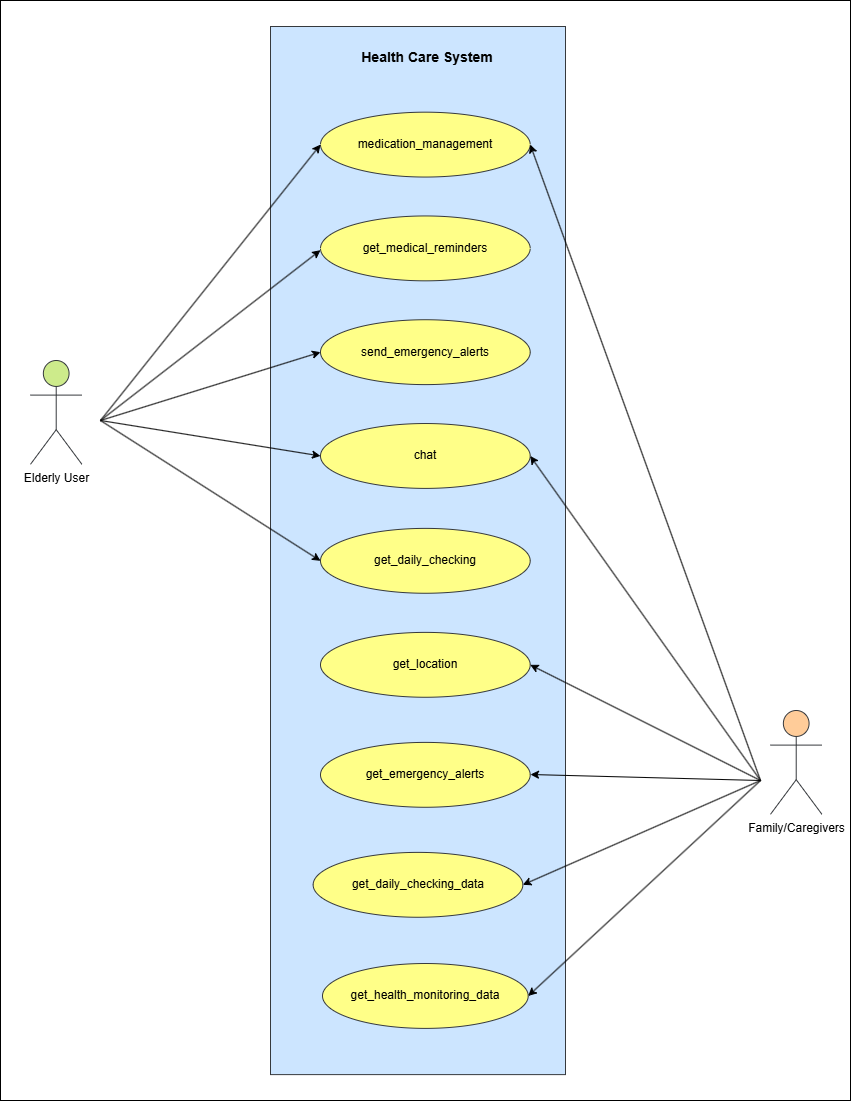
\includegraphics[width=0.5\linewidth]{usecase3.drawio (1).png}
    \caption{Enter Caption}
    \label{fig:enter-label}
\end{figure}

\newpage
\section{\textbf{\LARGE Implementation Plan}}

\subsection{\textbf{\Large 4.1 Introduction}}
ElderCare Connect is a Progressive Web App (PWA) designed to improve the safety, health monitoring, and social engagement of elderly individuals living alone. The app enables real-time health tracking, emergency alerts, and fosters social connections to combat loneliness among the elderly. With features like integration with Google Fit, emergency call APIs, and push notifications, the app aims to offer a comprehensive solution for elderly care.  
The app is available across multiple devices (smartphones, tablets, and desktops) without requiring installation, ensuring accessibility for elderly users who may have limited technical knowledge. Through this project, we aim to create a solution that enhances the well-being of elderly people, provides peace of mind to their families, and ensures prompt emergency response when necessary.

\subsection{\textbf{\Large 4.2 Importance of Implementation}}
The implementation phase is the most critical in turning the conceptual design of ElderCare Connect into a fully functioning app. It is at this stage where the app's core features are developed, tested, and optimized for real-world use. Effective implementation ensures that the app is functional, secure, and scalable, fulfilling its purpose of supporting elderly individuals.  
This phase involves integrating various technologies and services, such as health tracking with wearable devices, push notifications for emergencies, and secure authentication with JWT. It also includes rigorous system testing to detect and fix any issues before deployment. The implementation of these features directly impacts user experience, reliability, and the app's ability to meet its intended goals.

\section{\textbf{\LARGE Implementation Methodology}}

The development of ElderCare Connect followed an Agile methodology, which allowed for iterative development and continuous feedback from stakeholders. The project was broken down into smaller, manageable tasks that were completed in sprints, ensuring that each feature was developed, tested, and integrated step by step. This approach allowed the team to make improvements based on real-time feedback and user testing.

\begin{itemize}
    \item \textbf{Sprint 1:} Requirements gathering and setup of the development environment.
    \item \textbf{Sprint 2:} Frontend development (UI/UX design, layout creation using Next.js and Tailwind CSS).
    \item \textbf{Sprint 3:} Backend development (API setup with Node.js and Express, Firebase integration for real-time notifications).
    \item \textbf{Sprint 4:} Integration of real-time health monitoring (Google Fit).
    \item \textbf{Sprint 5:} Security implementation (JWT authentication, SSL encryption).
    \item \textbf{Sprint 6:} Testing, deployment, and final refinements based on user feedback.
\end{itemize}

\section{\textbf{\LARGE Implementation Environment}}

The implementation environment for ElderCare Connect consists of various tools and technologies that support both frontend and backend development.

\subsection*{Frontend:}
\begin{itemize}
    \item \textbf{Next.js:} Chosen for its ability to build server-side rendered React applications, making the app more SEO-friendly and performant.
    \item \textbf{Tailwind CSS:} A utility-first CSS framework that enabled rapid design implementation.
\end{itemize}

\subsection*{Backend:}
\begin{itemize}
    \item \textbf{Node.js:} The backend is built with Node.js due to its non-blocking, event-driven architecture, making it ideal for real-time data handling.
    \item \textbf{Express.js:} A web application framework for Node.js, used to handle routing and middleware for API requests.
    \item \textbf{MongoDB/Firebase:} MongoDB is used for storing user data and health records, while Firebase handles real-time notifications and authentication.
\end{itemize}

\subsection*{Other Tools:}
\begin{itemize}
    \item \textbf{Git:} Version control system for team collaboration.
    \item \textbf{Postman:} Used for API testing during development.
    \item \textbf{Firebase Cloud Messaging (FCM):} For sending push notifications, emergency alerts, and real-time medication reminders.
    \item \textbf{Jest:} A testing framework used to ensure that the backend APIs function as expected.
\end{itemize}

\section{\textbf{\LARGE Tools Used}}

\subsection*{Frontend:}
\begin{itemize}
    \item \textbf{Next.js:} Framework for building React-based web applications.
    \item \textbf{Tailwind CSS:} Used for creating responsive and modern designs.
    \item \textbf{Figma:} Design tool for UI/UX wireframing and prototyping.
\end{itemize}

\subsection*{Backend:}
\begin{itemize}
    \item \textbf{Node.js:} JavaScript runtime for the server-side environment.
    \item \textbf{Express.js:} Web framework for building APIs.
    \item \textbf{MongoDB/Firebase:} Database management (MongoDB for storing data, Firebase for real-time notifications and authentication).
    \item \textbf{JWT:} JSON Web Token used for secure authentication.
\end{itemize}

\subsection*{Testing:}
\begin{itemize}
    \item \textbf{Jest:} For unit and integration testing.
    \item \textbf{Postman:} For testing the backend API endpoints.
\end{itemize}

\subsection*{Version Control:}
\begin{itemize}
    \item \textbf{Git:} Used for source code management and version control, with GitHub for collaboration.
\end{itemize}

\section{\textbf{\LARGE System Testing}}

System testing was carried out to ensure that the ElderCare Connect app functions as expected under various conditions. The testing process included:

\begin{itemize}
    \item \textbf{Unit Testing:} Testing individual components like the login system, emergency alerts, and API endpoints using Jest.
    \item \textbf{Integration Testing:} Ensuring that components such as the frontend, backend, and Firebase service work seamlessly together.
    \item \textbf{User Acceptance Testing (UAT):} Involving actual users to test the app’s usability and gather feedback on its features and design.
    \item \textbf{Performance Testing:} Checking the app's ability to handle real-time notifications and large datasets without delays.
    \item \textbf{Security Testing:} Ensuring that data, especially health-related data, is securely transmitted using SSL encryption, and verifying the robustness of JWT-based authentication.
\end{itemize}

\section{\textbf{\LARGE Technical Stack}}

\begin{itemize}
    \item \textbf{Frontend:} Next.js, Tailwind CSS
    \item \textbf{Backend:} Node.js, Express.js
    \item \textbf{Database:} MongoDB, Firebase
    \item \textbf{Real-Time Services:} Firebase Cloud Messaging (FCM), WebSockets
    \item \textbf{Authentication:} JWT (JSON Web Token)
    \item \textbf{Security:} SSL encryption
    \item \textbf{Testing Tools:} Jest, Postman
    \item \textbf{Version Control:} Git, GitHub
    \item \textbf{Deployment:} Firebase Hosting
\end{itemize}

\end{document}
